\PassOptionsToPackage{landscape}{geometry}
\documentclass[aspectratio=43]{beamer}

\usetheme{default}
\usecolortheme{owl}

\setbeamerfont{frametitle}{series=\bfseries}
\setbeamercolor{frametitle}{fg=white,bg=black}

\setbeamerfont{framesubtitle}{size=\normalfont\tiny}
\setbeamercolor{framesubtitle}{fg=white}


\usepackage{bm}

\def\IC{\mathbb{C}}
\def\IF{\mathbb{F}}
\def\II{\mathbb{I}}
\def\IM{\mathbb{M}}
\def\IN{\mathbb{N}}
\def\IP{\mathbb{P}}
\def\IR{\mathbb{R}}
\def\IZ{\mathbb{Z}}

\def\ba{\mathbf{a}}
\def\bb{\mathbf{b}}
\def\bc{\mathbf{c}}
\def\be{\mathbf{e}}
\def\bh{\mathbf{h}}
\def\bi{\mathbf{i}}
\def\bj{\mathbf{j}}
\def\bk{\mathbf{k}}
\def\bn{\mathbf{n}}
\def\bp{\mathbf{p}}
\def\br{\mathbf{r}}
\def\bs{\mathbf{s}}
\def\bu{\mathbf{u}}
\def\bv{\mathbf{v}}
\def\bw{\mathbf{w}}
\def\bx{\mathbf{x}}
\def\by{\mathbf{y}}
\def\bz{\mathbf{z}}

\def\bB{\mathbf{B}}
\def\bD{\mathbf{D}}
\def\bF{\mathbf{F}}
\def\bG{\mathbf{G}}
\def\bN{\mathbf{N}}
\def\bR{\mathbf{R}}
\def\bS{\mathbf{S}}
\def\bT{\mathbf{T}}
\def\b0{\mathbf{0}}

\def\A{\mathcal{A}}
\def\B{\mathcal{B}}
\def\C{\mathcal{C}}
\def\D{\mathcal{D}}
\def\E{\mathcal{E}}
\def\F{\mathcal{F}}
\def\G{\mathcal{G}}
\def\I{\mathcal{I}}
\def\L{\mathcal{L}}
\def\M{\mathcal{M}}
\def\P{\mathcal{P}}
\def\R{\mathcal{R}}
\def\S{\mathcal{S}}
\def\T{\mathcal{T}}
\def\U{\mathcal{U}}
\def\V{\mathcal{V}}

\def\cov{\ensuremath{\mathsf{cov}}}
\def\Var{\ensuremath{\mathsf{Var}\ }}

\newtheorem{proposition}[theorem]{Proposition}
\newtheorem{property}[theorem]{Property}
\newtheorem{importantproperty}[theorem]{Property}
\newtheorem{importanttheorem}[theorem]{Theorem}
%\newtheorem{lemma}[theorem]{Lemma}



\setbeamertemplate{navigation symbols}{}
\setbeamertemplate{footline}
{%
	\quad\insertsection\hfill p. \insertpagenumber\quad\mbox{}\vskip2pt
}
\usecolortheme{orchid}
\setbeamertemplate{theorems}[numbered]

%%%%%%%% 
%%% Definitions in yellow boxes
\usepackage{etoolbox}
%\setbeamercolor{block title}{use=structure,fg=structure.fg,bg=structure.fg!20!bg}
%\setbeamercolor{block body}{parent=normal text,use=block title,bg=block title.bg!50!bg}
%
\BeforeBeginEnvironment{definition}{%
	\setbeamercolor{block title}{fg=blue,bg=black}
	\setbeamercolor{block body}{fg=white, bg=black!95!white}
}
\AfterEndEnvironment{definition}{
	\setbeamercolor{block title}{use=structure,fg=structure.fg,bg=structure.fg!20!bg}
	\setbeamercolor{block body}{parent=normal text,use=block title,bg=block title.bg!50!bg, fg=black}
}
\BeforeBeginEnvironment{theorem}{%
	\setbeamercolor{block title}{fg=green,bg=black}
	\setbeamercolor{block body}{fg=white, bg=black!95!white}
}
\AfterEndEnvironment{theorem}{
	\setbeamercolor{block title}{use=structure,fg=structure.fg,bg=structure.fg!20!bg}
	\setbeamercolor{block body}{parent=normal text,use=block title,bg=block title.bg!50!bg, fg=black}
}
%\BeforeBeginEnvironment{importanttheorem}{%
%	\setbeamercolor{block title}{fg=black,bg=red!50!white}
%	\setbeamercolor{block body}{fg=black, bg=red!30!white}
%}
%\AfterEndEnvironment{importanttheorem}{
%	\setbeamercolor{block title}{use=structure,fg=structure.fg,bg=structure.fg!20!bg}
%	\setbeamercolor{block body}{parent=normal text,use=block title,bg=block title.bg!50!bg, fg=black}
%}
%\BeforeBeginEnvironment{importantproperty}{%
%	\setbeamercolor{block title}{fg=black,bg=red!50!white}
%	\setbeamercolor{block body}{fg=black, bg=red!30!white}
%}
%\AfterEndEnvironment{importantproperty}{
%	\setbeamercolor{block title}{use=structure,fg=structure.fg,bg=structure.fg!20!bg}
%	\setbeamercolor{block body}{parent=normal text,use=block title,bg=block title.bg!50!bg, fg=black}
%}




\title{Principal Component Analysis (PCA)}
\date{}

\begin{document}
\DeclareFontShape{OT1}{cmss}{b}{n}{<->ssub * cmss/bx/n}{} 
\begin{frame}
	\titlepage
\end{frame}


%%%%%%%%%%%%%%%%%%%%%
%%%%%%%%%%%%%%%%%%%%%
%%%%%%%%%%%%%%%%%%%%%
%%%%%%%%%%%%%%%%%%%%%


\begin{frame}{Dimensionality reduction}
One of the reasons the SVD is used is for dimensionality reduction. However, SVD has many many other uses
\vfill
Now we look at another dimensionality reduction technique, PCA
\vfill
PCA is often used as a blackbox technique, here we take a look at the math behind it
\end{frame}


\begin{frame}{What is PCA?}
Linear algebraic technique 
\vfill
Helps reduce a complex dataset to a lower dimensional one
\vfill
Non-parametric method: does not assume anything about data distribution (distribution from the statistical point of view)
\end{frame}


\begin{frame}{Brief ``review'' of some probability concepts}
Proper definition of \emph{probability} requires to use \emph{measure theory}.. will not get into details here
\vfill
A \textbf{random variable} $X$ is a \emph{measurable} function $X:\Omega\to E$, where $\Omega$ is a set of outcomes (\emph{sample space}) and $E$ is a measurable space
\vfill
$\IP(X\in S\subseteq E) = \IP(\omega\in\Omega|X(\omega)\in S)$
\vfill
\textbf{Distribution function} of a r.v., $F(x)=\IP(X\leq x)$, describes the distribution of a r.v.
\vfill
R.v. can be discrete or continuous or .. other things. 
\end{frame}

\begin{frame}
\begin{definition}[Variance]
Let $X$ be a random variable. The \textbf{variance} of $X$ is given by
\[
\Var X = E\left[\left(X-E(X)\right)^2\right]
\]
where $E$ is the expected value
\end{definition}
\vfill
\begin{definition}[Covariance]
Let $X,Y$ be jointly distributed random variables. The \textbf{covariance} of $X$ and $Y$ is given by
\[
\cov (X,Y) = E\left[\left(X-E(X)\right)\left(Y-E(Y)\right)\right]
\]
\end{definition}
\vfill
Note that $\cov(X,X)=E\left[\left(X-E(X)\right)^2\right] = \Var X$
\end{frame}

\begin{frame}{In practice: ``true law'' versus ``observation''}
In statistics: we reason on the \emph{true law} of distributions, but we usually have only access to a sample
\vfill
We then use \textbf{estimators} to .. estimate the value of a parameter, e.g., the mean, variance and covariance
\vfill
\end{frame}
	
\begin{frame}
\begin{definition}[Unbiased estimators of the mean and variance]
Let $x_1,\ldots,x_n$ be data points (the \emph{sample}) and 
\[
\bar x = \frac 1n \sum_{i=1}^n x_i
\]
be the \textbf{mean} of the data. An unbiased estimator of the variance of the sample is
\[
\sigma^2 = \frac{1}{n-1}\sum_{i=1}^n (x_i-\bar x)^2
\]
\end{definition}
\end{frame}

\begin{frame}
\begin{definition}[Unbiased estimator of the covariance]
Let $(x_1,y_1),\ldots,(x_n,y_n)$ be data points,
\[
\bar x = \frac 1n \sum_{i=1}^n x_i
\textrm{ and }
\bar y = \frac 1n \sum_{i=1}^n y_i
\]
be the means of the data. An estimator of the covariance of the sample is
\[
\cov(x,y) = \frac{1}{n}\sum_{i=1}^n (x_i-\bar x)(y_i-\bar y)
\]
\end{definition}
\end{frame}

\begin{frame}{What does covariance do?}
Variance explains how data disperses around the mean, in a 1-D case
\vfill
Covariance measures the relationship between two dimensions. E.g., height and weight
\vfill
More than the exact value, the sign is important:
\begin{itemize}
	\item $\cov(X,Y)>0$: both dimensions change in the same ``direction''; e.g., larger height usually means higher weight
	\item $\cov(X,Y)<0$: both dimensions change in reverse directions; e.g., time spent on social media and performance in this class
	\item $\cov(X,Y)=0$: the dimensions are independent from one another; e.g., sex/gender and ``intelligence''
\end{itemize}
\end{frame}

\begin{frame}{The covariance matrix}
Typically, we consider more than 2 variables.. 
\begin{definition}
Suppose $p$ random variables $X_1,\ldots,X_p$. Then the covariance matrix is the symmetric matrix
\[
\begin{pmatrix}
\cov(X_1,X_1) & \cov(X_1,X_2) & \cdots & \cov(X_1,X_p) \\
\cov(X_2,X_1) & \cov(X_2,X_2) & \cdots & \cov(X_2,X_p) \\
\vdots & \vdots & & \vdots \\
\cov(X_p,X_1) & \cov(X_p,X_2) & \cdots & \cov(X_p,X_p) 
\end{pmatrix}
\]
i.e., using the properties of covariance,
\[
\begin{pmatrix}
\Var X_1 & \cov(X_1,X_2) & \cdots & \cov(X_1,X_p) \\
\cov(X_1,X_2) & \Var X_2 & \cdots & \cov(X_2,X_p) \\
\vdots & \vdots & & \vdots \\
\cov(X_1,X_p) & \cov(X_2,X_p) & \cdots & \Var X_p 
\end{pmatrix}
\]
\end{definition}
\end{frame}


\begin{frame}{Example of a PCA problem}
We collect a bunch of information about a bunch of people.. for instance this data from Loughborough University
\vfill
\begin{quote}
This dataset contains the height, weight and 4 fingerprint measurements (length, width, area and circumference), collected from 200 participants.
\end{quote}
\vfill
What best describes a participant?
\end{frame}

\begin{frame}{The variables}
Each participant is associated to 11 variables
\vfill
\begin{itemize}
\item "Participant Number"
\item "Gender"
\item "Age"
\item "Dominant Hand"
\item "Height (cm) (average of 3 measurements)"
\item "Weight (kg) (average of 3 measurements)"
\item "Fingertip Temperature (°C)"
\item "Fingerprint Height (mm)"
\item "Fingerprint Width (mm)"
\item "Fingerprint Area (mm2)"
\item "Fingerprint Circumference (mm)"
\end{itemize}
\end{frame}

\begin{frame}{Nature of variables}
Variables have different natures
\vfill
\begin{itemize}
\item "Participant Number": $\in\IN$ (not interesting)
\item "Gender": categorical
\item "Age": $\in\IN$ 
\item "Dominant Hand": categorical
\item "Height (cm) (average of 3 measurements)": $\in\IR$
\item "Weight (kg) (average of 3 measurements)": $\in\IR$
\item "Fingertip Temperature (°C)": $\in\IR$
\item "Fingerprint Height (mm)": $\in\IR$
\item "Fingerprint Width (mm)": $\in\IR$
\item "Fingerprint Area (mm2)": $\in\IR$
\item "Fingerprint Circumference (mm)": $\in\IR$
\end{itemize}
\end{frame}

\begin{frame}{Setting things up}
Each participant is a row in the matrix (an \emph{observation})
\vfill
Each variable is a column
\vfill
So we have an $200\times 10$ matrix (we discard the ``Participant number'' column)
\vfill
We want to find what carries the most information
\vfill
For this, we are going to project the information in a new basis in which the first ``dimension'' will carry most variance, the second dimension will carry a little less, etc.
\vfill
In order to do so, we need to learn how to change bases
\end{frame}



\begin{frame}{Change of basis}
\begin{definition}[Change of basis matrix]
$\B=\{\bu_1,\ldots,\bu_n\}$ and $\C=\{\bv_1,\ldots,\bv_n\}$ bases of vector space $V$
\vskip0.2cm
The \textbf{change of basis matrix} $P_{\C\leftarrow\B}\in\M_n$,
\[
P_{\C\leftarrow\B}
=\left[
[\bu_1]_\C \cdots [\bu_n]_\C
\right]
\]
has columns the coordinate vectors $[\bu_1]_\C,\ldots,[\bu_n]_\C$ of the vectors in $\B$ with respect to $\C$
\end{definition}
\vfill
\begin{theorem}
$\B=\{\bu_1,\ldots,\bu_n\}$ and $\C=\{\bv_1,\ldots,\bv_n\}$ bases of vector space $V$ and $P_{\C\leftarrow\B}$ a change of basis matrix from $\B$ to $\C$
\begin{enumerate}
\item $\forall\bx\in V$, $P_{\C\leftarrow\B}[\bx]_\B = [\bx]_\C$
\item $P_{\C\leftarrow\B}$ s.t. $\forall\bx\in V$, $P_{\C\leftarrow\B}[\bx]_\B = [\bx]_\C$ is \textbf{unique}
\item $P_{\C\leftarrow\B}$ invertible and $P_{\C\leftarrow\B}^{-1}=P_{\B\leftarrow\C}$
\end{enumerate}
\end{theorem}
\end{frame}


\begin{frame}{Row-reduction method for changing bases}
\begin{theorem}
$\B=\{\bu_1,\ldots,\bu_n\}$ and $\C=\{\bv_1,\ldots,\bv_n\}$ bases of vector space $V$. Let $\E$ be any basis for $V$,
\[
B = [[\bu_1]_\E,\ldots,[\bu_n]_\E] 
\textrm{ and }
C = [[\bv_1]_\E,\ldots,[\bv_n]_\E] 
\]
and let $[C|B]$ be the augmented matrix constructed using $C$ and $B$. Then
\[
RREF\left([C|B]\right)
=[\II|P_{\C\leftarrow\B}]
\]
\end{theorem}
\vfill
If working in $\IR^n$, this is quite useful with $\E$ the standard basis of $\IR^n$ (it does not matter if $\B=\E$)
\end{frame}

\begin{frame}
So the question now becomes
\begin{quote}
How do we find what new basis to look at our data in?
\end{quote}
\vfill
(Changing the basis does not change the data, just the view you have of it)
\vfill
(Think of what happens when you do a headstand.. your up becomes down, your right and left switch, but the world does not change, just your view of it)
\vfill
(Changes of bases are \emph{fundamental} operations in Science)
\end{frame}



\begin{frame}{Setting things up}
I will use notation (mostly) as in Joliffe's \emph{Principal Component Analysis} (PDF of older version available for free from UofM Libraries)
\vfill
$\bx=(x_1,\ldots,x_p)$ vector of $p$ random variables
\end{frame}


\begin{frame} 
We seek a linear function $\bm{\alpha}_1^T\bx$ with maximum variance, where $\bm{\alpha}_1=(\alpha_{11},\ldots,\alpha_{1p})$, i.e.,
\[
\bm{\alpha}_1^T\bx = \sum_{j=1}^p\alpha_{1j}x_j
\]
\vfill
Then we seek a linear function $\bm{\alpha}_2^T\bx$ with maximum variance, uncorrelated to $\bm{\alpha}_1^T\bx$
\vfill
And we continue...
\vfill
At $k$th stage, we find a linear function $\bm{\alpha}_k^T\bx$ with maximum variance, uncorrelated to $\bm{\alpha}_1^T\bx,\ldots,\bm{\alpha}_{k-1}^T\bx$
\vfill
$\bm{\alpha}_i^T\bx$ is the $i$th \textbf{principal component} (PC)
\end{frame}

\begin{frame}{Case of known covariance matrix}
Suppose we know $\Sigma$, covariance matrix of $\bx$ (i.e., typically: we know $\bx$)
\vfill
Then the $k$th PC is 
\[
z_k=\bm{\alpha}_k^T\bx
\]
where $\bm{\alpha}_k$ is an eigenvector of $\Sigma$ corresponding to the $k$th largest eigenvalue $\lambda_k$
\vfill
If, additionally, $\|\bm{\alpha}_k\|=\bm{\alpha}_k^T\bm{\alpha}=1$, then $\lambda_k=\Var z_k$
\end{frame}


\begin{frame}{Why is that?}
Let us start with
\[
\bm{\alpha}_1^T\bx
\]
\vfill
We want maximum variance, where $\bm{\alpha}_1=(\alpha_{11},\ldots,\alpha_{1p})$, i.e.,
\[
\bm{\alpha}_1^T\bx = \sum_{j=1}^p\alpha_{1j}x_j
\]
with the constraint that $\|\bm{\alpha}_1\|=1$
\vfill
We have
\[
\Var \bm{\alpha}_1^T\bx
=\bm{\alpha}_1^T\Sigma\bm{\alpha}_1
\]
\end{frame}

\begin{frame}{Objective}
We want to maximise $\Var \bm{\alpha}_1^T\bx$, i.e.,
\[
\bm{\alpha}_1^T\Sigma\bm{\alpha}_1
\]
under the constraint that $\|\bm{\alpha}_1\|=1$
\vfill
$\implies$ use \textbf{Lagrange multipliers}
\end{frame}


\begin{frame}{Maximisation using Lagrange multipliers}
\framesubtitle{(A.k.a. super-brief intro to multivariable calculus)}
We want the max of $f(x_1,\ldots,x_n)$ under the constraint $g(x_1,\ldots,x_n)=k$
\begin{enumerate}
\item Solve
\begin{align*}
\nabla f(x_1,\ldots,x_n) &= \lambda\nabla g(x_1,\ldots,x_n) \\
g(x_1,\ldots,x_n) &= k
\end{align*}
where $\nabla=(\frac{\partial}{\partial x_1},\ldots,\frac{\partial}{\partial x_n})$ is the \textbf{gradient operator}
\item Plug all solutions into $f(x_1,\ldots,x_n)$ and find maximum values (provided values exist and $\nabla g\neq \b0$ there)
\end{enumerate}
\vfill
$\lambda$ is the \textbf{Lagrange multiplier}
\end{frame}


\begin{frame}{The gradient}
\framesubtitle{(Continuing our super-brief intro to multivariable calculus)}
$f:\IR^n\to\IR$ function of several variables, $\nabla=\left(\frac{\partial}{\partial x_1},\ldots,\frac{\partial}{\partial x_n}\right)$ the gradient operator
\vfill
Then
\[
\nabla f = \left(
\frac{\partial}{\partial x_1}f,\ldots,
\frac{\partial}{\partial x_n}f
\right)
\]
\vfill
So $\nabla f$ is a \emph{vector-valued} function, $\nabla f:\IR^n\to\IR^n$; also written as
\[
\nabla f = f_{x_1}(x_1,\ldots,x_n)\be_1+\cdots f_{x_n}(x_1,\ldots,x_n)\be_n
\]
where $f_{x_i}$ is the partial derivative of $f$ with respect to $x_i$ and $\{\be_1,\ldots,\be_n\}$ is the standard basis of $\IR^n$
\end{frame}


\begin{frame}{Bear with me..}
\framesubtitle{(You may experience a brief period of discomfort)}
$\bm{\alpha}_1^T\Sigma\bm{\alpha}_1$ and $\|\bm{\alpha}_1\|^2=\bm{\alpha}_1^T\bm{\alpha_1}$ are functions of $\bm{\alpha}_1=(\alpha_{11},\ldots,\alpha_{1p})$
\vfill
In the notation of the previous slide, we want the max of 
\[
f(\alpha_{11},\ldots,\alpha_{1p}) := \bm{\alpha}_1^T\Sigma\bm{\alpha}_1
\]
under the constraint that
\[
g(\alpha_{11},\ldots,\alpha_{1p}) := \bm{\alpha}_1^T\bm{\alpha_1} = 1
\]
and with gradient operator
\[
\nabla = \left(
\frac{\partial}{\partial \alpha_{11}},
\ldots,
\frac{\partial}{\partial \alpha_{1p}}
\right)
\]
\end{frame}


\begin{frame}{Effect of $\nabla$ on $g$}
$g$ is easiest to see:
\begin{align*}
\nabla g(\alpha_{11},\ldots,\alpha_{1p}) &=
\left(
\frac{\partial}{\partial \alpha_{11}},
\ldots,
\frac{\partial}{\partial \alpha_{1p}}
\right) (\alpha_{11},\ldots,\alpha_{1p}) 
\begin{pmatrix}
\alpha_{11}\\ \vdots\\ \alpha_{1p}
\end{pmatrix} \\
&= \left(
\frac{\partial}{\partial \alpha_{11}},
\ldots,
\frac{\partial}{\partial \alpha_{1p}}
\right) 
\left(
\alpha_{11}^2+\cdots+\alpha_{1p}^2
\right) \\
&= \left(2\alpha_{11},\ldots,2\alpha_{1p}\right)\\
&= 2\bm{\alpha}_1
\end{align*}
\vfill
(And that's a general result: $\nabla\|\bx\|_2^2=2\bx$ with $\|\cdot\|_2$ the Euclidean norm)
\end{frame}

\begin{frame}{Effect of $\nabla$ on $f$}
Expand (write $\Sigma=[s_{ij}]$ and do not exploit symmetry)
\begin{align*}
\bm{\alpha}_1^T\Sigma\bm{\alpha}_1 &=
\left(\alpha_{11},\ldots,\alpha_{1p}\right)
\begin{pmatrix}
s_{11} & s_{12} & \cdots & s_{1p} \\
s_{21} & s_{22} & \cdots & s_{2p} \\
\vdots & \vdots & & \vdots \\
s_{p1} & s_{p2} & & s_{pp}
\end{pmatrix}
\begin{pmatrix}
\alpha_{11} \\ \alpha_{12} \\ \vdots \\ \alpha_{1p}
\end{pmatrix} \\
&=
\left(\alpha_{11},\ldots,\alpha_{1p}\right)
\begin{pmatrix}
s_{11}\alpha_{11}+s_{12}\alpha_{12}+\cdots+s_{1p}\alpha_{1p} \\
s_{21}\alpha_{11}+s_{22}\alpha_{12}+\cdots+s_{2p}\alpha_{1p} \\
\vdots \\
s_{p1}\alpha_{11}+s_{p2}\alpha_{12}+\cdots+s_{pp}\alpha_{1p}
\end{pmatrix} \\
&=
(s_{11}\alpha_{11}+s_{12}\alpha_{12}+\cdots+s_{1p}\alpha_{1p})\alpha_{11} \\
&\quad +
(s_{21}\alpha_{11}+s_{22}\alpha_{12}+\cdots+s_{2p}\alpha_{1p})\alpha_{12} \\
&\quad\;\;\vdots \\
&\quad +
(s_{p1}\alpha_{11}+s_{p2}\alpha_{12}+\cdots+s_{pp}\alpha_{1p})\alpha_{1p}
\end{align*}
\end{frame}

\begin{frame}
We have
\begin{align*}
\bm{\alpha}_1^T\Sigma\bm{\alpha}_1 &=
(s_{11}\alpha_{11}+s_{12}\alpha_{12}+\cdots+s_{1p}\alpha_{1p})\alpha_{11} \\
&\quad +
(s_{21}\alpha_{11}+s_{22}\alpha_{12}+\cdots+s_{2p}\alpha_{1p})\alpha_{12} \\
&\quad\;\;\vdots \\
&\quad +
(s_{p1}\alpha_{11}+s_{p2}\alpha_{12}+\cdots+s_{pp}\alpha_{1p})\alpha_{1p} 
\end{align*}
So
\begin{align*}
\frac{\partial}{\partial \alpha_{11}}
\bm{\alpha}_1^T\Sigma\bm{\alpha}_1  
&= 
(s_{11}\alpha_{11}+s_{12}\alpha_{12}+\cdots+s_{1p}\alpha_{1p})+s_{11}\alpha_{11} \\
&\quad +
s_{21}\alpha_{12} \\
&\quad\;\;\vdots \\
&\quad +
s_{p1}\alpha_{1p} \\
&= s_{11}\alpha_{11}+s_{12}\alpha_{12}+\cdots+s_{1p}\alpha_{1p} \\
&\quad+
s_{11}\alpha_{11}+s_{21}\alpha_{12}+\cdots+s_{p1}\alpha_{1p} \\
&= 2(s_{11}\alpha_{11}+s_{12}\alpha_{12}+\cdots+s_{1p}\alpha_{1p})
\end{align*}
(last equality stems from symmetry of $\Sigma$)
\end{frame}

\begin{frame}
In general, for $i=1,\ldots,p$,
\begin{align*}
\frac{\partial}{\partial \alpha_{1i}}
\bm{\alpha}_1^T\Sigma\bm{\alpha}_1  
&= s_{i1}\alpha_{11}+s_{i2}\alpha_{12}+\cdots+s_{ip}\alpha_{1p}\\
&\quad+s_{i1}\alpha_{11}+s_{2i}\alpha_{12}+\cdots+s_{pi}\alpha_{1p} \\
&= 2(s_{i1}\alpha_{11}+s_{i2}\alpha_{12}+\cdots+s_{ip}\alpha_{1p})
\end{align*}
(because of symmetry of $\Sigma$)
\vfill
As a consequence,
\[
\nabla \bm{\alpha}_1^T\Sigma\bm{\alpha}_1
=2\Sigma\bm{\alpha}_1
\]
\end{frame}

\begin{frame}
So solving
\[
\nabla f(x_1,\ldots,x_n) = \lambda\nabla g(x_1,\ldots,x_n) 
\]
means solving
\[
2\Sigma\bm{\alpha}_1 = \lambda 2\bm{\alpha}_1 
\]
i.e.,
\[
\Sigma\bm{\alpha}_1 = \lambda\bm{\alpha}_1 
\]
\vfill
$\implies$
$(\lambda,\bm{\alpha}_1)$ eigenpair of $\Sigma$, with $\bm{\alpha}_1$ having unit length
\end{frame}


\begin{frame}{Picking the right eigenvalue}
$(\lambda,\bm{\alpha}_1)$ eigenpair of $\Sigma$, with $\bm{\alpha}_1$ having unit length
\vfill
But which $\lambda$ to choose?
\vfill
Recall that we want $\Var \bm{\alpha}_1^T\bx=\bm{\alpha}_1^T\Sigma\bm{\alpha}_1$ maximal
\vfill
We have
\[
\Var \bm{\alpha}_1^T\bx 
= \bm{\alpha}_1^T\Sigma\bm{\alpha}_1 
= \bm{\alpha}_1^T(\Sigma\bm{\alpha}_1) 
= \bm{\alpha}_1^T(\lambda\bm{\alpha}_1) 
= \lambda(\bm{\alpha}_1^T\bm{\alpha}_1) = \lambda
\]
\vfill
$\implies$ we pick $\lambda=\lambda_1$, the largest eigenvalue (covariance matrix symmetric so eigenvalues real)
\end{frame}


\begin{frame}{What we have this far..}
The first principal component is $\bm{\alpha}_1^T\bx$ and has variance $\lambda_1$, where $\lambda_1$ the largest eigenvalue of $\Sigma$ and $\bm{\alpha}_1$ an associated eigenvector with $\|\bm{\alpha}_1\|=1$
\vfill
We want the second principal component to be \emph{uncorrelated} with $\bm{\alpha}_1^T\bx$ and to have maximum variance $\Var \bm{\alpha}_2^T\bx=\bm{\alpha}_2^T\Sigma\bm{\alpha}_2$, under the constraint that $\|\bm{\alpha}_2\|=1$
\vfill
$\bm{\alpha}_2^T\bx$ uncorrelated to $\bm{\alpha}_1^T\bx$ if $\cov(\bm{\alpha}_1^T\bx,\bm{\alpha}_2^T\bx)=0$
\end{frame}

\begin{frame}
We have
\begin{align*}
\cov(\bm{\alpha}_1^T\bx,\bm{\alpha}_2^T\bx) &= 
\bm{\alpha}_1^T\Sigma\bm{\alpha}_2 \\
&= \bm{\alpha}_2^T\Sigma^T\bm{\alpha}_1 \\
&= \bm{\alpha}_2^T\Sigma\bm{\alpha}_1 \quad\textrm{[$\Sigma$ symmetric]} \\
&= \bm{\alpha}_2^T(\lambda_1\bm{\alpha}_1) \\
&= \lambda \bm{\alpha}_2^T\bm{\alpha}_1
\end{align*}
\vfill
So $\bm{\alpha}_2^T\bx$ uncorrelated to $\bm{\alpha}_1^T\bx$ if $\bm{\alpha}_1\perp\bm{\alpha}_2$
\vfill
This is beginning to sound a lot like Gram-Schmidt, no?
\end{frame}

\begin{frame}{In short}
Take whatever covariance matrix is available to you (known $\Sigma$ or sample $S_X$) -- assume sample from now on for simplicity
\vfill
For $i=1,\ldots,p$, the $i$th principal component is
\[
z_i = \bv_i^T\bx
\]
where $\bv_i$ eigenvector of $S_X$ associated to the $i$th largest eigenvalue $\lambda_i$
\vfill
If $\bv_i$ is normalised, then $\lambda_i=\Var z_k$
\end{frame}


\begin{frame}{Covariance matrix}
$\Sigma$ the covariance matrix of the random variable, $S_X$ the sample covariance matrix
\vfill
$X\in\M_{mp}$ the data, then the (sample) covariance matrix $S_X$ takes the form
\[
S_X = \frac{1}{n-1}X^TX
\]
where the data is centred!
\vfill
Sometimes you will see $S_X=1/(n-1)XX^T$. This is for matrices with observations in columns and variables in rows. Just remember that you want the covariance matrix to have size the number of variables, not observations, this will give you the order in which to take the product
\end{frame}

\begin{frame}{A smaller 2D example}
	\framesubtitle{Hockey players at IIHF world championships 2001-2016}
	\begin{center}
		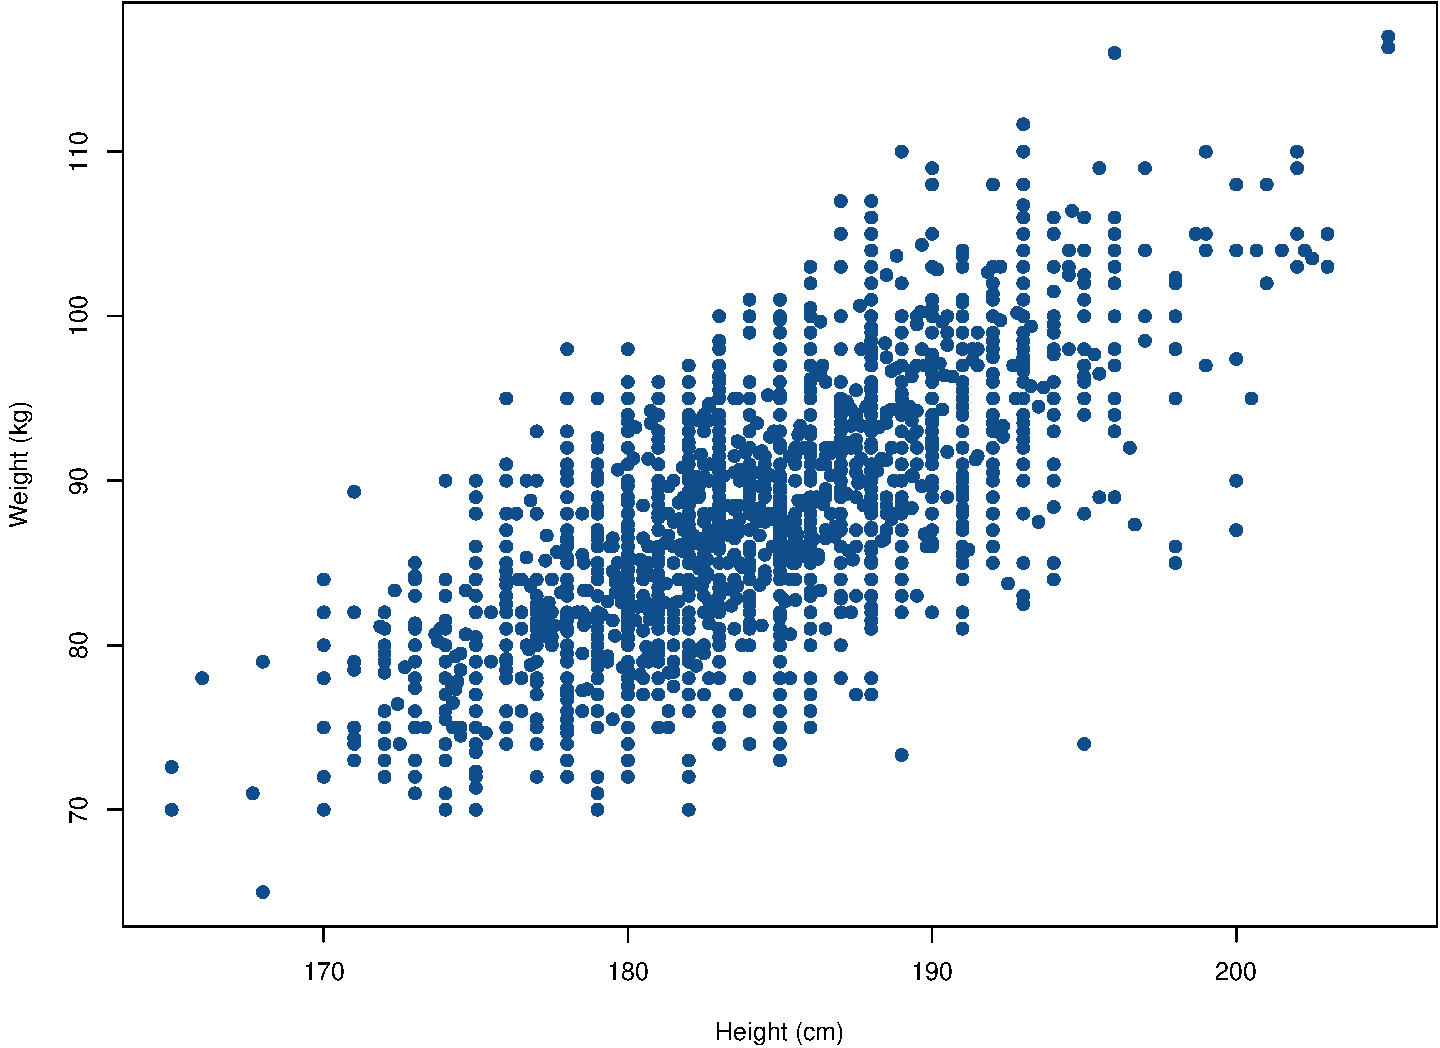
\includegraphics[height=0.85\textheight]{FIGS_slides/slides-08-hockey_players_raw}
	\end{center}
\end{frame}

\begin{frame}{Centre the data}
	\framesubtitle{Subtract the mean (our first -- simple -- change of basis)}
	\begin{center}
		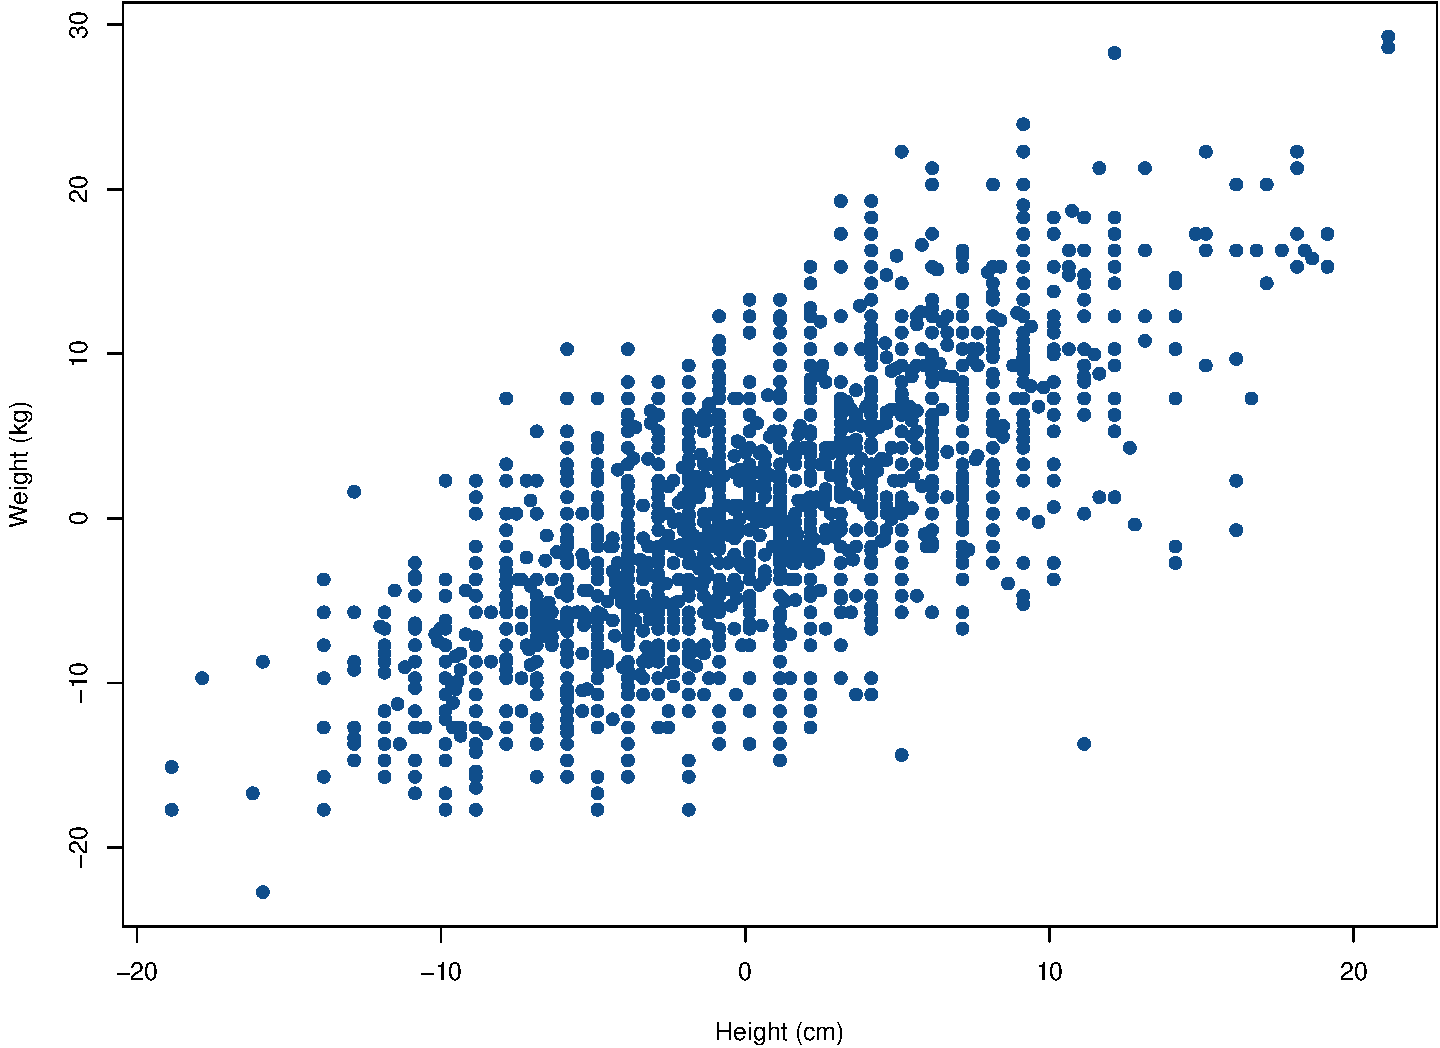
\includegraphics[height=0.85\textheight]{FIGS_slides/slides-08-hockey_players_centred}
	\end{center}
\end{frame}


\end{document}
